% ------------------------------------------------------------------------------
% TYPO3 Version 10.1 - What's New (English Version)
%
% @author	Michael Schams <schams.net>
% @license	Creative Commons BY-NC-SA 3.0
% @link		http://typo3.org/download/release-notes/whats-new/
% @language	English
% ------------------------------------------------------------------------------

\section{Backend User Interface}
\begin{frame}[fragile]
	\frametitle{Backend User Interface}

	\begin{center}\huge{Chapter 1:}\end{center}
	\begin{center}\huge{\color{typo3darkgrey}\textbf{Backend User Interface}}\end{center}

\end{frame}

% ------------------------------------------------------------------------------
% Feature | 89115 | Auto slug update and redirect creation on slug change

\begin{frame}[fragile]
	\frametitle{Backend User Interface}
	\framesubtitle{Slug Updates and Redirects (1)}

	\begin{itemize}
		\item When backend users change the URL path of a page (the so-called "slug"),
			the old URL becomes unavailable.
		\item This possibly results in a "page not found" error for this page,
			including the URLs of all sub-pages.
	\end{itemize}

	\begin{figure}
		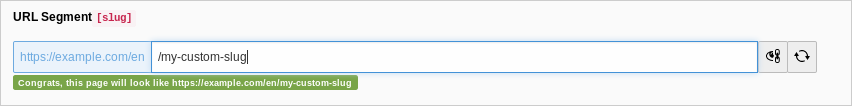
\includegraphics[width=0.80\linewidth]{BackendUserInterface/89115b-AutoSlugUpdateAndRedirectCreationOnSlugChange.png}
	\end{figure}

	\begin{itemize}
		\item Since TYPO3 v10.1, two actions prevent this from happening:

			\begin{itemize}
				\item slugs for all sub-pages are automatically updated
				\item redirects from the old to the new URLs are created
			\end{itemize}

	\end{itemize}

\end{frame}

% ------------------------------------------------------------------------------
% Feature | 89115 | Auto slug update and redirect creation on slug change

\begin{frame}[fragile]
	\frametitle{Backend User Interface}
	\framesubtitle{Slug Updates and Redirects (2)}

	\begin{itemize}
		\item Backend users are informed about these actions and they can
			easily roll back the changes with a click of a button if required:

	\end{itemize}

	\begin{figure}
		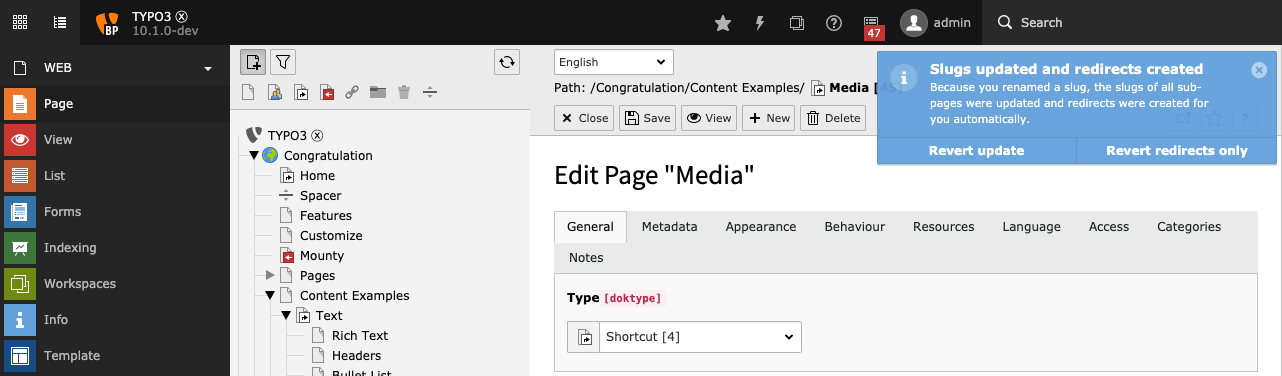
\includegraphics[width=0.80\linewidth]{BackendUserInterface/89115c-AutoSlugUpdateAndRedirectCreationOnSlugChange.png}
	\end{figure}

\end{frame}

% ------------------------------------------------------------------------------
% Feature | 85918 | Hide in menu / Show in menu entry for pages in context menu

\begin{frame}[fragile]
	\frametitle{Backend User Interface}
	\framesubtitle{Hide/Show in Menu}

	A new entry was added to the context menu to show/hide pages in the menu.

	\begin{figure}
		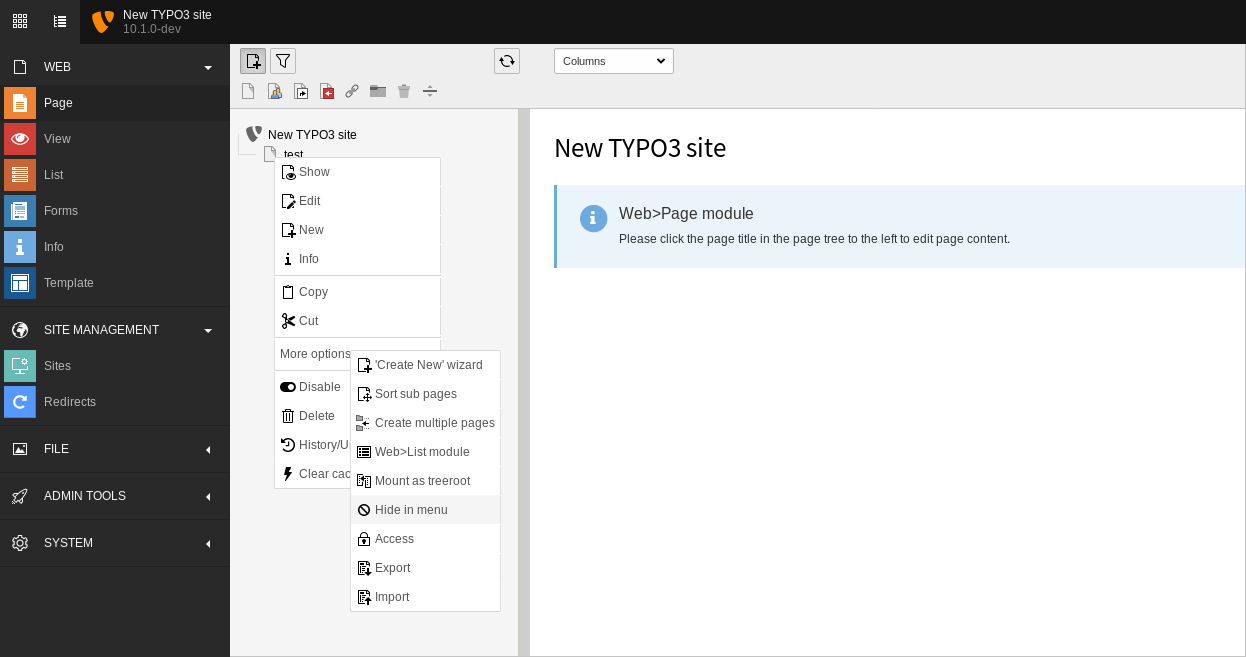
\includegraphics[width=0.80\linewidth]{BackendUserInterface/85918-HideShowInMenu-InContextMenu.png}
	\end{figure}

\end{frame}

% ------------------------------------------------------------------------------
